\documentclass[10pt,letterpaper]{article} 
%\usepackage{tikz}
\usepackage{amsmath,amssymb,geometry}
%\usepackage{graphicx}‎‎
%\usefonttheme{serif}‎
%\usepackage{ptext}‎
\usepackage{xepersian}
%\settextfont{B Nazanin}
\usepackage{lipsum}
\setlength{\parindent}{0pt}
%\usepackage{enumitem}
%\setlist[enumerate,1]{label=(\arabic*)}
\newcommand{\pf}{$\blacksquare$}
\newcommand{\EX}{\Bbb E}
\newcommand{\nl}{\newline\newline}
\setlength{\parskip}{1em}

\usepackage{amsmath}
\usepackage{accents}
\newlength{\dhatheight}
\newcommand{\doublehat}[1]{%
    \settoheight{\dhatheight}{\ensuremath{\hat{#1}}}%
    \addtolength{\dhatheight}{-0.35ex}%
    \hat{\vphantom{\rule{1pt}{\dhatheight}}%
    \smash{\hat{#1}}}}

\newcounter{QuestionNumber}
\setcounter{QuestionNumber}{1}

\newcommand{\Q}{
\textbf{
سوال \theQuestionNumber)
}
\stepcounter{QuestionNumber}
}

\newcommand{\fig}[3]{
\begin{figure}[h!]
#1
\caption{#2}
\label{#3}
\end{figure}
}

\newcommand{\subfig}[3]{
\begin{subfigure}{#3}
#1
\caption{#2}
\end{subfigure}
}
%\newcommand{\pic}[2]{
%\begin{center}
%\includegraphics[width=#2]{#1}
%\end{center}
%}
\begin{document}
\Large
\begin{center}
به نام زیبایی

تمرینات سری دهم سیگنال ها و سیستم ها

\hrulefill
\end{center}
%\Q
%
%تبدیل فوریه‌ی سیگنال های زمان گسسته‌ی زیر را به دست آورید.
%
%الف)
%$
%x[n]=u[n]-u[n-5]
%$
%
%ب)
%$
%x[n]=({1\over 3})^nu[n]
%$
%
%پ)
%$
%x[n]=-({1\over 3})^nu[-n-1]
%$
%
%ت)
%$
%x[n]=\sin{\pi\over 2}n+\cos n
%$
%
%ث) 
%$
%x[n]=n({1\over 3})^nu[n]
%$
%
%\Q
%
%عکس تبدیل فوریه‌ی سیگنال های زیر را به دست آورید.
%
%الف)
%$
%X(e^{j\omega})=\sum_{k=-\infty}^{\infty}(-1)^k\delta(\omega-{\pi\over 2}k)
%$
%
%ب)
%$
%X(e^{j\omega})={1-{1\over 3}e^{-j\omega}\over 1-{1\over 4}e^{-j\omega}-{1\over 8}e^{-2j\omega}}
%$
%
%پ) 
%$
%X(e^{j\omega})={1\over 1-e^{-4j\omega}}
%$

\large

\Q

اگر $x[n]$ دارای تبدیل فوریه‌ی 
$
X(e^{j\omega})
$
 باشد، تبدیل فوریه‌ی سیگنال های زیر را بر حسب
$
X(e^{j\omega})
$
بنویسید.

الف)
$
y[n]=x[-1-n]+x[1-n]
$

ب)
$
y[n]={x^*[-n]+x[n]\over 2}
$

پ)
$
y[n]=(n-1)^2x[n]
$


\Q

فرض کنید 
$
X(e^{j\omega})
$
 تبدیل فوریه‌ی سیگنال زیر باشد:
\begin{figure}[h!]
\centering
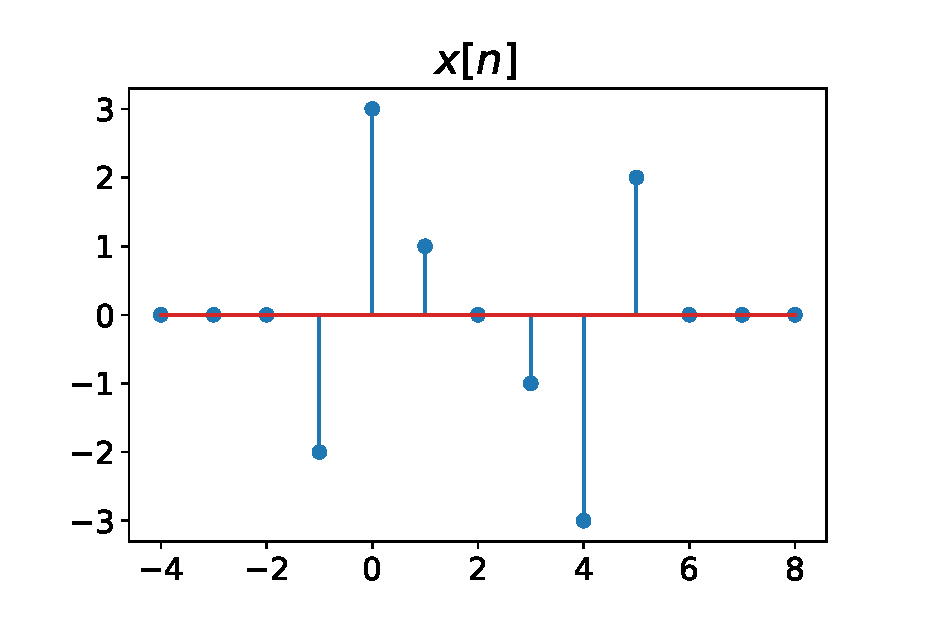
\includegraphics[width=90mm]{Q12_Final.eps}
\end{figure}

در این صورت، موارد زیر را به کمک خواص تبدیل فوریه و بدون محاسبه مستقیم آن بیابید:

%الف)
%$
%X(e^{j0})
%$

الف)
$
\measuredangle X(e^{j\omega})
$

ب)
$
\int_{-\pi}^{\pi} X(e^{j\omega})d\omega
$

پ)
$
X(e^{j\pi})
$
%
%ث)
%$
%\int_{-\pi}^{\pi} |X(e^{j\omega})|^2d\omega
%$

ت)
$
\int_{-\pi}^{\pi} \left|{dX(e^{j\omega})\over d\omega}\right|^2d\omega
$

%چ) سیگنالی که تبدیل فوریه‌ی آن 
%$
%\Re\{X(e^{j\omega})\}
%$
% باشد.


\Q

فرض کنید اطلاعات زیر در خصوص یک سیستم LTI با پاسخ فرکانسی 
$
H(e^{j\omega})
$
 و پاسخ ضربه‌ی 
$
h[n]
$
 داده شده است:

$\blacksquare$
$({1\over 4})^nu[n]\longrightarrow g[n]$ 
که در آن 
$
g[n]=0
$
اگر $n<0$ یا $n\ge 2$

$\blacksquare$
$H(e^{j{\pi\over 2}})=1$

$\blacksquare$
$H(e^{j\omega})=H(e^{j(\omega-\pi)})$

در این صورت 
$
h[n]
$
 را بیابید.

%\Q
%
%سیستم LTI ای را در نظر بگیرید که از سری کردن دو سیستم زیر به دست آمده است:
%$$
%H_1(e^{j\omega})={2-e^{-j\omega}\over 1+{1\over 2}e^{-j\omega}}
%$$
%و
%$$
%H_1(e^{j\omega})={1\over 1-{1\over 2}e^{-j\omega}+{1\over 4}e^{-j2\omega}}
%$$
%در این صورت:
%
%الف)
%معادله‌ی تفاضلی سیستم کلی را بیابید.
%
%ب) پاسخ ضربه‌ی سیستم کلی را بیابید.

%\Q
%
%یک سیستم LTI، دارای معادله تفاضلی زیر است:
%$$
%y[n]-ay[n-1]=bx[n]+x[n-1]
%$$
%که در آن، 
%$
%a\in \Bbb R
%$
% و 
%$
%|a|<1
%$.
%
%الف) مقدار $b$ را چنان بیابید به گونه ای که
%$$
%|H(e^{j\omega})|=1\quad,\quad \text{ برای هر $\omega$}
%$$
% به چنین سیستمی تمام گذر می گویند؛ زیرا هیچ تضعیفی روی دامنه‌ی فرکانسی سیگنال ورودی اعمال نمی‌کند. از مقدار $b$ به دست آمده در این قسمت، برای بخش های بعدی بهره ببرید.
%
%ب) به طور تقریبی، 
%$
%\measuredangle H(e^{j\omega})
%$
% را به ازای
%$
%a={1\over 2}
%$
% رسم کنید.
%
%پ) به طور تقریبی، 
%$
%\measuredangle H(e^{j\omega})
%$
% را به ازای
%$
%a=-{1\over 2}
%$
% رسم کنید.
%
%ت)
% خروجی این سیستم را به ورودی 
%$
%x[n]=({1\over 2})^nu[n]
%$
% زمانی که
%$
%a=-{1\over 2}
%$
% به دست آورده و رسم کنید. 
%
%از این مثال می توان دید که یه اثر غیرخطی در فاز در مقایسه با شیفت فاز خطی، می تواند اثر متفاوتی بر حوزه‌ی زمان سیگنال بر جا گذارد.

\Q

یک سیستم LTI با پاسخ ضربه‌ی $h[n]$ و پاسخ فرکانسی 
$
H(e^{j\omega})
$
 دارای این خاصیت است که برای هر 
$
-\pi\le \omega_0\le \pi
$
:
$$
\cos \omega_0 n\longrightarrow \omega_0\cos \omega_0n
$$
در این صورت:

الف)
$
H(e^{j\omega})
$
 را بیابید.

ب)
$
h[n]
$
 را بیابید.

\Q

برای هر یک از گزاره‌های زیر، درستی یا نادرستی آن را با بیان دلیل تعیین کنید.

الف)
$$
X(e^{j\omega})=X(e^{j(\omega-1)})\implies x[n]=0\quad,\quad |n|>0
$$

ب)
$$
X(e^{j\omega})=X(e^{j(\omega-\pi)})\implies x[n]=0\quad,\quad |n|>0
$$

پ)
$$
X(e^{j\omega})=X(e^{j{\omega\over 2}})\implies x[n]=0\quad,\quad |n|>0
$$

ت)
$$
X(e^{j\omega})=X(e^{j2\omega})\implies x[n]=0\quad,\quad |n|>0
$$

\Q

الف) 
سیستمی با ورودی $x[n]$ و خروجی $y[n]$ مفروض است. تبدیل‌ فوریه‌ی این دو سیگنال با رابطه‌ی زیر به هم مربوط می شوند:
$$
Y(e^{j\omega})=2X(e^{j\omega})+e^{-j\omega}X(e^{j\omega})-{dX(e^{j\omega})\over d\omega}
$$
الف-1) آیا این سیستم خطی است؟ تغییر ناپذیر با زمان چطور؟

الف-2) پاسخ این سیستم به ورودی 
$
x[n]=\delta[n]
$
 چیست؟

ب) فرض کنید رابطه‌ی ورودی و خروجی یک سیستم در حوزه‌ی فرکانس به صورت زیر داده شده است:
$$
Y(e^{j\omega})=\int_{\omega-{\pi\over 4}}^{\omega+{\pi\over 4}}X(e^{j\omega})d\omega
$$
رابطه‌ی ورودی و خروجی این سیستم در حوزه‌ی زمان چیست؟

%\Q
%
%خواص زیر را از تبدیل فوریه‌ی گسسته نشان دهید!
%
%اگر سیگنال $x[n]$ دارای تبدیل فوریه‌ی 
%$
%X(e^{j\omega})
%$
% باشد، ثابت کنید:
%
%الف)
%$$
%nx[n]\implies j{dX(e^{j\omega})\over d\omega}
%$$
%ب) 
%$$
%\sum_{k=-\infty}^{n}x[k]\implies {1\over 1-e^{-j\omega}}X(e^{j\omega})+
%\pi X(e^{j0})\sum_{k=-\infty}^{\infty}\delta(\omega-2\pi k)
%$$
%پ) اگر $x[n]$ حقیقی باشد، آنگاه:
%$$
%X(e^{j\omega})=X^*(e^{-j\omega})
%$$
%و 
%$
%\Re\{X(e^{j\omega})\}
%$
%، معادل تبدیل فوریه‌ی قسمت زوج سیگنال حقیقی و 
%$
%\Im\{X(e^{j\omega})\}
%$
% معادل تبدیل فوریه‌ی قسمت فرد سیگنال حقیقی است.
%
%ت) اتحاد پارسوال:
%$$
%\sum_{n=-\infty}^{\infty}|x[n]|^2={1\over 2\pi}\int_{-\pi}^{\pi}|X(e^{j\omega})|^2d\omega
%$$
%ث) دوگانی: سیگنال 
%$
%y(t)=X(e^{jt})
%$
%متناوب با دوره‌ی $2\pi$ و دارای ضرایب سری فوریه‌ی گسسته‌ی 
%$
%x[-n]
%$
% است.
\end{document}